% based on https://vtex-soft.github.io/texsupport.isba-ba/
% \documentclass[ba,preprint]{imsart}% use this for supplement article
\documentclass[ba]{imsart}

\pubyear{\the\year{}}
\volume{TBA}
\issue{TBA}
\doi{10.31219/osf.io/wh3wr}
\arxiv{2010.010101}
\firstpage{1}
\lastpage{1}

%
\usepackage{amsthm}
\usepackage{amsmath}
\usepackage{natbib}
\usepackage[colorlinks,citecolor=blue,urlcolor=blue,filecolor=blue,backref=page]{hyperref}
\usepackage{graphicx}

\startlocaldefs
\numberwithin{equation}{section}
\theoremstyle{plain}
\newtheorem{thm}{Theorem}[section]
\endlocaldefs
% rticles required

% tightlist command for lists without linebreak
\providecommand{\tightlist}{%
  \setlength{\itemsep}{0pt}\setlength{\parskip}{0pt}}

% From pandoc table feature
\usepackage{longtable,booktabs,array}
\usepackage{calc} % for calculating minipage widths
% Correct order of tables after \paragraph or \subparagraph
\usepackage{etoolbox}
\makeatletter
\patchcmd\longtable{\par}{\if@noskipsec\mbox{}\fi\par}{}{}
\makeatother
% Allow footnotes in longtable head/foot
\IfFileExists{footnotehyper.sty}{\usepackage{footnotehyper}}{\usepackage{footnote}}
\makesavenoteenv{longtable}


% Pandoc header

\begin{document}
\begin{frontmatter}

\title{Short Paper for Bayesian Analyis}
\runtitle{Short Paper for Bayesian Analyis}

\begin{aug}
\author{Alice Anonymous\thanksref{addr1,t1,t2,m1}\ead[label=ea-1,email]{alice@example.com}\ead[label=ua-1,url]{www.example.com/aliceanon}}, \author{Bob Security\thanksref{addr1,t3,m1,m2}\ead[label=ea-2,email]{bob@example.com}}, \author{Cat Memes\thanksref{addr2,t1,m2}\ead[label=ea-3,email]{cat@example.com}}
\runauthor{Anonymous et al.}

 %loop through affiliations
\address[addr1]{Some Institute of Technology, Department, Street, City, State, Zip \ifstrequal{addr1}{addr1}{\printead{ea-1}}{}
\ifstrequal{addr1}{addr1}{\printead{ua-1}}{}
 \ifstrequal{addr1}{addr1}{\printead{ea-2}}{}
 \ifstrequal{addr1}{addr2}{\printead{ea-3}}{}
%authors
} %loop through affiliations
\address[addr2]{Another University, Department, Street, City, State, Zip \ifstrequal{addr2}{addr1}{\printead{ea-1}}{}
\ifstrequal{addr2}{addr1}{\printead{ua-1}}{}
 \ifstrequal{addr2}{addr1}{\printead{ea-2}}{}
 \ifstrequal{addr2}{addr2}{\printead{ea-3}}{}
%authors
}%affiliations

\thankstext{t1}{Corresponding Author}
\thankstext{t2}{Equal contribution}
\thankstext{t3}{Something}
\thankstext{m1}{Something}
\thankstext{m2}{Something}

\end{aug}

\begin{abstract}
The abstract should summarize the contents of the paper. It should be clear, descriptive, self-explanatory and not longer than 200 words. It should also be suitable for publication in abstracting services. Please avoid using math formulas as much as possible.

This is a sample input file. Comparing it with the output it generates can show you how to produce a simple document of your. That was the second paragraph.
\end{abstract}

% MSC class
 \begin{keyword}[class=MSC]
\kwd[Primary ]{62C10}
\kwd{62F15}
\kwd[; secondary ]{60K35}
\kwd{91A27}\end{keyword}
% keywords
 \begin{keyword} \kwd{bayesian} \kwd{statistics}\end{keyword}
\end{frontmatter}

\hypertarget{r-markdown}{%
\section{R Markdown}\label{r-markdown}}

This is an R Markdown document. Markdown is a simple formatting syntax for authoring HTML, PDF, and MS Word documents. For more details on using R Markdown see \url{http://rmarkdown.rstudio.com}.

When you click the \textbf{Knit} button a document will be generated that includes both content as well as the output of any embedded R code chunks within the document. You can embed an R code chunk like this:

\begin{verbatim}
summary(cars)
\end{verbatim}

\begin{verbatim}
##      speed           dist       
##  Min.   : 4.0   Min.   :  2.00  
##  1st Qu.:12.0   1st Qu.: 26.00  
##  Median :15.0   Median : 36.00  
##  Mean   :15.4   Mean   : 42.98  
##  3rd Qu.:19.0   3rd Qu.: 56.00  
##  Max.   :25.0   Max.   :120.00
\end{verbatim}

\hypertarget{yaml-fields}{%
\subsection{YAML fields}\label{yaml-fields}}

For \texttt{MSC2020primary} and \texttt{MSC2020secondary}, please refer to \href{https://mathscinet.ams.org/mathscinet/msc/msc2020.html}{MSC database}.

\hypertarget{including-plots}{%
\subsection{Including Plots}\label{including-plots}}

You can also embed plots, for example:

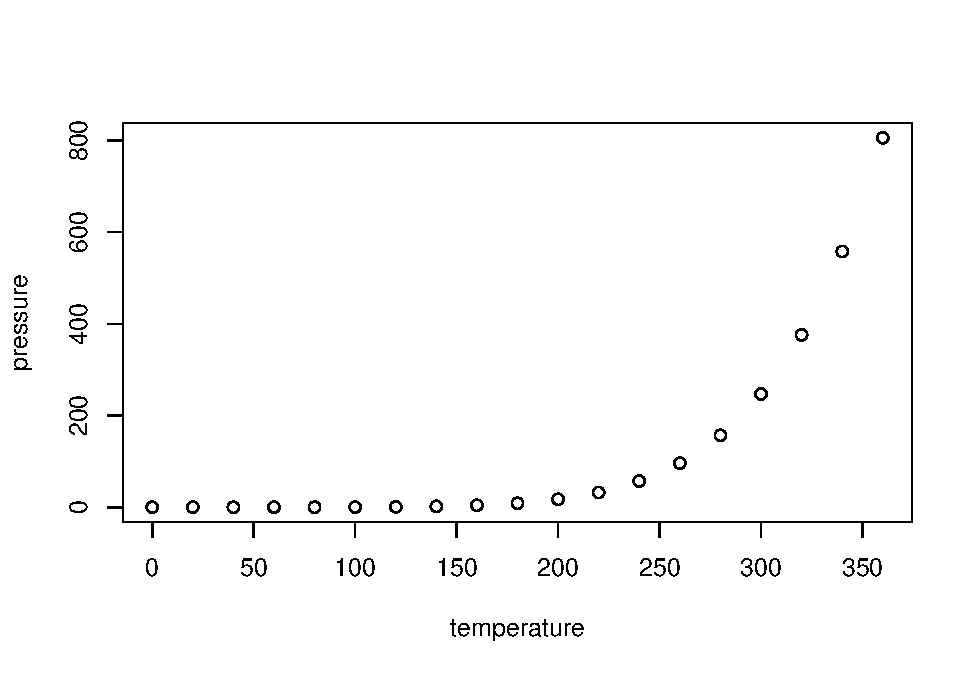
\includegraphics{Untitled_files/figure-latex/pressure-1.pdf}

Note that the \texttt{echo\ =\ FALSE} parameter was added to the code chunk to prevent printing of the R code that generated the plot. Because printing is different from typewriting, there are a number of things that you have to do differently when preparing an input file than if you were just typing the document directly. Quotation marks separates the double and single quote.

\[a+b\geq c\]
where \(a\) is a variable and \(c\) is variable as well.

Dashes come in three sizes: a hyphen, an intra-word dash, a medium dash for number ranges like 1--2, and a punctuation dash in place of a comma, semicolon, colon or parentheses ---like this.

The following are some other citations to check that the bibliographic style file is working correctly: \citet{akaike}, \citet*{akivarsq},
\citet*{kstuart}, and \citet{companion}.

\begin{supplement}
\stitle{Title of Supplement A}
\sdescription{Short description of Supplement A.}
\end{supplement}
\begin{supplement}
\stitle{Title of Supplement B}
\sdescription{Short description of Supplement B.}
\end{supplement}

\begin{acks}[Acknowledgments]
And this is an acknowledgements section with a heading that was produced by the \texttt{acks} environment. Thank you all for helping me writing this Rmarkdown sample file.

Also thankful to God, mom and my cats.
\end{acks}

\bibliographystyle{ba}
\bibliography{sample.bib}


\end{document}
